% Условная компиляция для самостоятельной работы
\ifdefined\mainfile
    % Если это часть основного файла, не добавляем начало и конец документа
\else
    \documentclass[12pt, a4paper]{report}
    \usepackage{/Users/vladbelousov/Desktop/Semestr_4-FP-NSU/Настройка/library}
    \usepackage[utf8]{inputenc} % Подключение поддержки UTF-8
    \begin{document}
\fi

%%-------------------------------%%
\[ \lambda_1, \ldots, \lambda_n \text{  - собственные числа матрицы } A  \] 

\begin{theorem}
    Нулевое решение \( \vec{y } ^* (t )= 0\) системы (2) асимптотически устойчиво \( \Leftrightarrow  \forall  \lambda_1, \ldots, \lambda_n :  \mathrm{Re } \lambda_j < 0 , \text{ }  j=1, \ldots, n \).
\end{theorem}

\begin{proof} \(  \) 

    \( (\Rightarrow): \)

    От противного. Пусть \( \exists  \lambda_k : \mathrm{Re } \lambda_k \ge  0  \). Взять решение \( \vec{y } (t ) =  e^{ \lambda_k t } \vec{v }_k , \text{ }  \vec{v } _k \) - собственный вектор, соответственного \( \lambda_k \). 

    \[ \left\lVert  \vec{y } (t) \right\rVert = \left\lVert e^{\lambda_k t } \vec{v } _k   \right\rVert = \left\lvert e^{ \lambda_k t }  \right\rvert \left\lVert  \vec{v }  _k  \right\rVert  = e^{\mathrm{Re } \lambda_k t  } \underbrace{\left\lVert \vec{v } _k  \right\rVert}_{\neq 0} \cancel{\xrightarrow{ t \to  +\infty }} 0    \] 
    \( \Rightarrow \) нулевое решение не асимптотически устойчиво. Противоречие \( \Rightarrow  \forall  \lambda_j \text{ }  \mathrm{Re }  \lambda_j < 0  \) 

    \( (\Leftarrow): \) 

    Пусть \( \forall  \lambda_j \text{ }  \mathrm{Re }  \lambda_j < 0   \). Все решения системы \( \vec{y } (t ) = c_1 \vec{\varphi }_1 (t )+ ... + c_n \vec{\varphi }_n (t)   \) 
    
    \[ \lambda_1 \to \underbrace{ \vec{v } _c , \vec{v } _{\text{ пр}_1 },...,  \vec{v } _{\text{ пр}_{m-1} }}_{m \text{ - векторов} }  \] 

    \[ \begin{aligned}
        \begin{cases}
            \vec{\varphi }_1 (t ) = e^{ \lambda_1 t } \vec{v } _{\text{ с} }  \\
            \vec{\varphi }_2  (t ) = e^{ \lambda_1t }(  \vec{v } _{\text{ с} }t +\vec{ v } _{\text{пр}_{1}}  )\\
            \vdots \\
            \vec{\varphi }_m (t ) = e^{ \lambda_1 t }  \left( \vec{v } _{\text{ с} } \frac{t ^{m-1 } }{(m-1 )! } +... + \vec{ v } _{\text{пр}_{m-2}   } t + \vec{v } _{\text{пр}_{m-1}  }    \right)
        \end{cases} 
        \begin{aligned}
        &\left\lVert \vec{\varphi }_1 (t) \right\rVert = \left\lvert e^{ \lambda_1 t }  \right\rvert \left\lVert \vec{ v } _{c}  \right\rVert = e^{ \mathrm{Re }  \lambda_j t } \left\lVert \vec{v } _c   \right\rVert \xrightarrow{t \to + \infty } 0   \\
        &\left\lVert \vec{\varphi }_2 (t) \right\rVert  = e^{ \mathrm{Re }  \lambda_j t } \left\lVert  \vec{v } _{\text{ с} }t +\vec{ v } _{\text{пр}_{1}} \right\rVert \xrightarrow{t \to + \infty } 0   \\
        &\vdots \\ 
        &\left\lVert \vec{\varphi }_m (t)  \right\rVert \xrightarrow{t \to  + \infty } 0  
        \end{aligned}
    \end{aligned}\] 

Дописать 

\( \Rightarrow \left\lVert \vec{y } (t ) \right\rVert \le  \left\lvert  c_1  \right\rvert \left\lVert \vec{\varphi }_1 (t)  \right\rVert + \left\lvert  c_n\right\rvert \left\lVert \vec{\varphi }_n (t)  \right\rVert \xrightarrow{t \to  + \infty } 0   \) \\

\end{proof}

\begin{theorem}
    Пусть \( \exists \lambda_k : \mathrm{Re }  \lambda_k > 0 \Rightarrow \vec{y}  ^ * (t ) = 0   \) неустойчиво.
\end{theorem}

\begin{proof} \(  \) 

    Смотреть доказательство Теоремы 3. \( (\Rightarrow) \) (Надо заменить \( \mathrm{Re }  \lambda_k \ge  0  \) на \( \mathrm{Re }  \lambda_k > 0  \))\\

\end{proof}

\begin{theorem}
    Пусть \( \forall  \lambda_j \text{ }  \mathrm{ Re }  \lambda_j \le  0   \) и \( \exists  \lambda_k : \mathrm{Re }  \lambda_k = 0  \). 

    1) Если \( \forall  \lambda_k : \mathrm{ Re } \lambda_k  = 0  \), у собственного числа \( \lambda_k \) нет присоединенных векторов, то \( \vec{y } ^* (t ) \) системы (2) устойчиво по Ляпунову; 

    2) Если \( \exists  \lambda_k : \mathrm{Re }  \lambda_k  =0   \), у собственного числа \( \lambda_k  \) есть присоединенные вектора, то \( \vec{y} ^{* } (t ) \) неустойчиво.
\end{theorem}

\begin{proof} \(  \) 

    1) Все решения системы: \( \vec{y } (t ) = c_1 \vec{\varphi }_1 (t )+...+ c_n \vec{\varphi }_n (t)   \) 

    \( \lambda_1, \ldots, \lambda_n : \mathrm{Re }  \lambda_k = 0  , \text{ }  k= 1, \ldots, m  \) 

    \( \lambda_{m+1 },..., \lambda_n : \mathrm{Re }  \lambda_j < 0 ,\text{ }  j = m+1 ,..., n   \) 

    \[ \begin{aligned}
        \begin{cases}
            \vec{\varphi }_1 (t ) = e^{ \lambda_1 t } \vec{v } _{c_1 }  \\
            \vec{\varphi }_2 (t ) = e^{ \lambda_2 t } \vec{ v }  _{c_2}  \\
            \vdots \\ 
            \vec{\varphi }_m (t ) = e^{ \lambda_m t } \vec{v }_{c_m }   
        \end{cases} 
        \left\lVert \vec{\varphi }_k (t)  \right\rVert = \underbrace{\left\lvert e^{\lambda_k t }  \right\rvert}_{=1} \left\lVert \vec{v } _{c_k }  \right\rVert = \left\lVert \vec{v }  _{c_k }  \right\rVert 
    \end{aligned}\] 

    \[ \vec{\varphi}  _{m+1 } (t ) ,..., \vec{\varphi } _n(t ) \xrightarrow{t \to  +\infty } 0    \] 

    \[ \Rightarrow \left\lVert \vec{y } (t ) \right\rVert \le  \left\lvert  c_1  \right\rvert \underbrace{\left\lVert  \vec{\varphi }_1 (t)  \right\rVert}_{\left\lVert \vec{v } _{c_1}  \right\rVert} +...+ \left\lvert c_m \right\rvert \underbrace{\left\lVert \vec{\varphi }_m(t)  \right\rVert}_{\left\lVert \vec{v } _{c_m}  \right\rVert} + \left\lvert c_{m+1 }    \right\rvert \underbrace{\left\lVert  \vec{\varphi }_{m+1 } (t )  \right\rVert}_{\xrightarrow{t \to  + \infty } 0} + \left\lvert c_n \right\rvert \underbrace{\left\lVert  \vec{\varphi }_n (t )  \right\rVert}_{\xrightarrow{t \to  + \infty } 0  } \] 

    Все решение ограничено вправо. 
    
    \(\Rightarrow \vec{y } ^* (t ) = 0  \)  устойчиво по Ляпунову

    2) \( \lambda_k: \mathrm{Re } \lambda_k = 0 \Rightarrow \vec{v } _k   \)  -собственное  вектор, \( \vec{v } _{\text{пр} }   \) - присоединенный вектор. 

    \[ \vec{y } (t ) = e^{ \lambda_k t } (\vec{v } _c (t ) + \vec{v } _{\text{пр}}  ) \text{ - решение}  \] 

    \[ \left\lVert \vec{y } (t) \right\rVert  = \left\lvert e^{ \lambda_k t }   \right\rvert \left\lVert \vec{v } _c (t ) + \vec{v } _{\text{пр}}   \right\rVert \ge  \left\lVert \vec{v } _c  \right\rVert \left\lvert t  \right\rvert - \left\lVert \vec{v  } _{\text{пр}}  \right\rVert   \xrightarrow{ t \to + \infty      } \infty   \] 
    \[ \vec{y } ^* (t ) = 0 \text{ - неустойчиво.}  \] 

\end{proof}

\section{Устойчивость решений автономных систем}

\[ \frac{d}{dt }  \vec{y } = \vec{ } (\vec{y } ) \tag{1} \] 

(1) - автономная система, так как \( \vec{f } (\vec{y } ) \) явно не зависит от \( t \). 

\[ \vec{y } = \begin{pmatrix}
y_1     \\
\vdots\\
y_n
\end{pmatrix} , \text{ }  \vec{f } (\vec{y }  ) = \begin{pmatrix}
f_1(\vec{y } ) \\
\vdots\\
f_n (\vec{y } ) 
\end{pmatrix} \] 

Выполняются условия теоремы Пикара, то есть \( \vec{f } (\vec{y} ) \) - непрерывен и \( \exists \displaystyle  \frac{\partial  f_i }{\partial  y_i}  \) - непрерывно.

\( \vec{y} ^* (t ) = 0  \) -  решение \( \Rightarrow \vec{0 }  = \vec{f } (\vec{0} )  \)

Пусть \( \vec{y } (t) \) - решение (1), определенно  при \( t \in  (\alpha , \omega) \) 

\begin{center}
    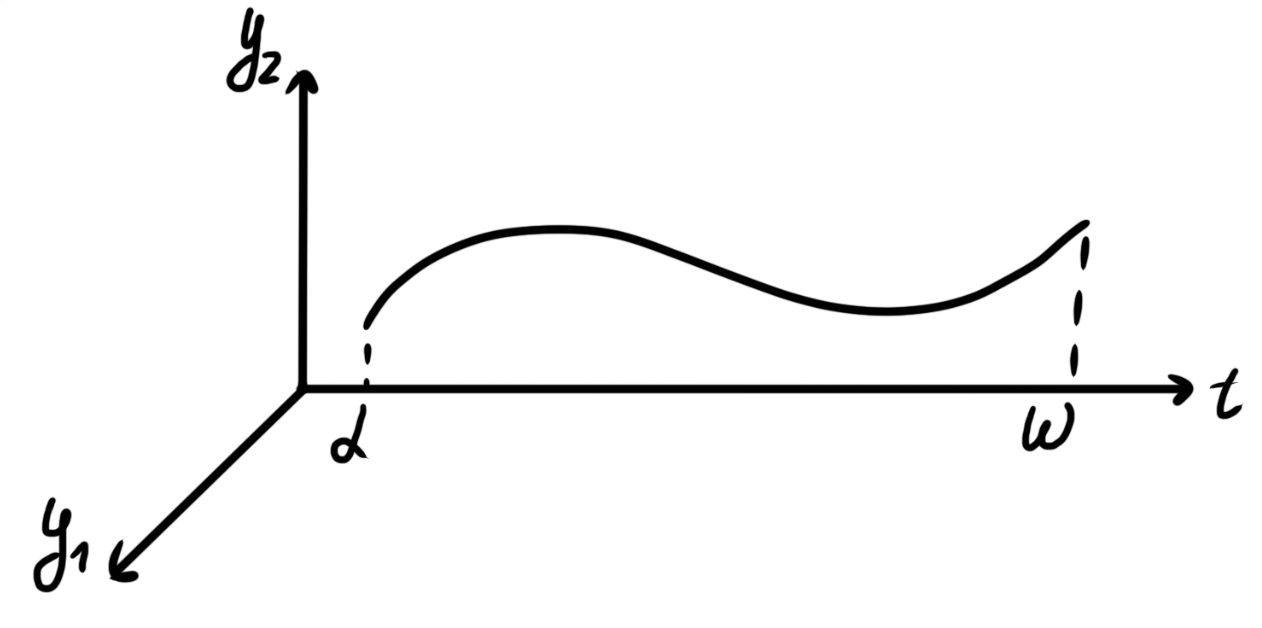
\includegraphics[width=0.6\textwidth]{/Users/vladbelousov/Desktop/Semestr_4-FP-NSU/ДфУ/Лекции_по_дням/image/45.png}
\end{center}

\textit{Интегральная кривая}  - график решения, то есть множество точек \( \{(t,y_1(t ),..., y_n(t)), t \in  (\alpha , \omega)\} \) 

\begin{center}
    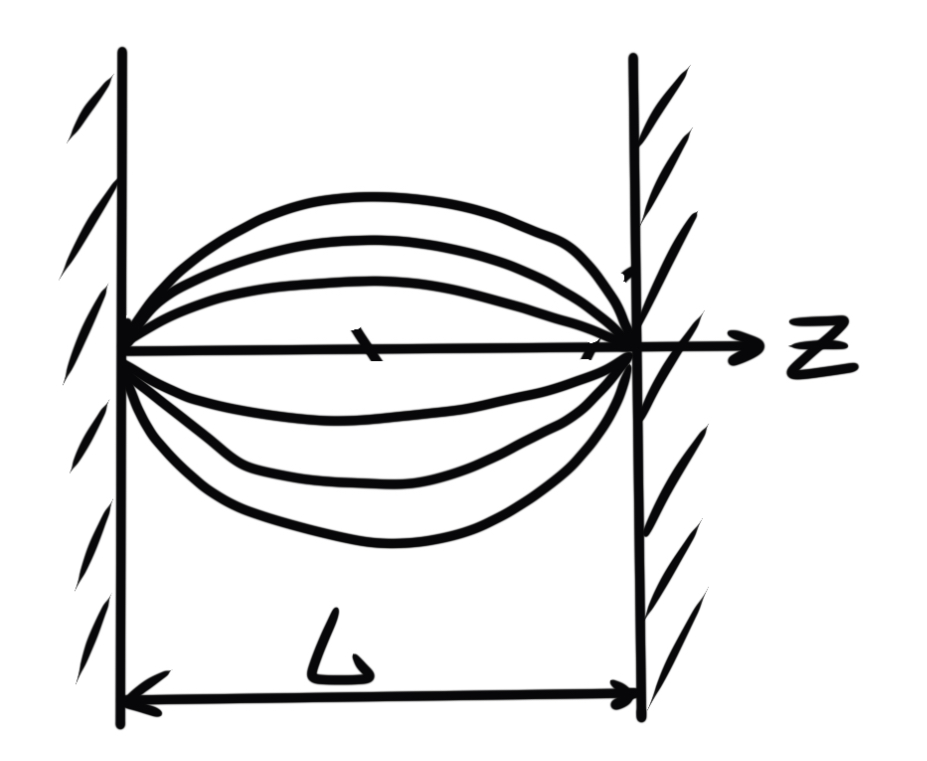
\includegraphics[width=0.4\textwidth]{/Users/vladbelousov/Desktop/Semestr_4-FP-NSU/ДфУ/Лекции_по_дням/image/46.png}
\end{center}

\textit{Фазовая траектория} - проекция интегральной кривой на пространство \( \{y_1, \ldots, y_n\} \), то есть множество точек \( \{(y_1, \ldots, y_n ) , t \in (\alpha , \omega)\} \) 

\textit{Фазовое пространство} - пространство \( \{y_1, \ldots, y_n\} \)  

Устойчивость нулевого решения: 

\begin{center}
    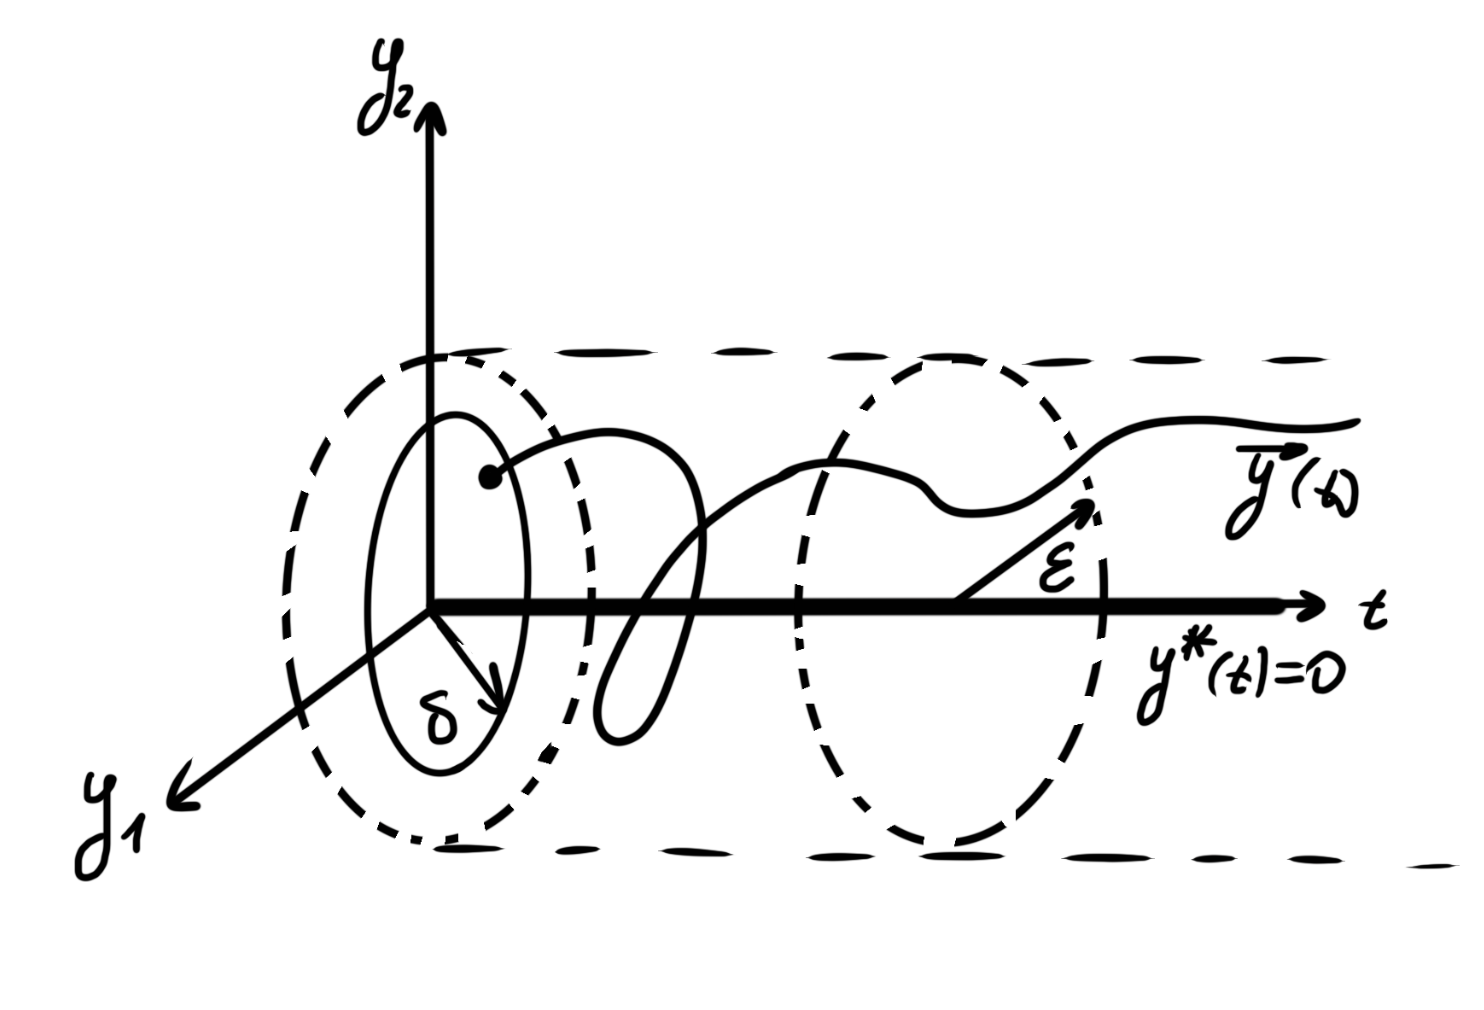
\includegraphics[width=0.6\textwidth]{/Users/vladbelousov/Desktop/Semestr_4-FP-NSU/ДфУ/Лекции_по_дням/image/47.png}
    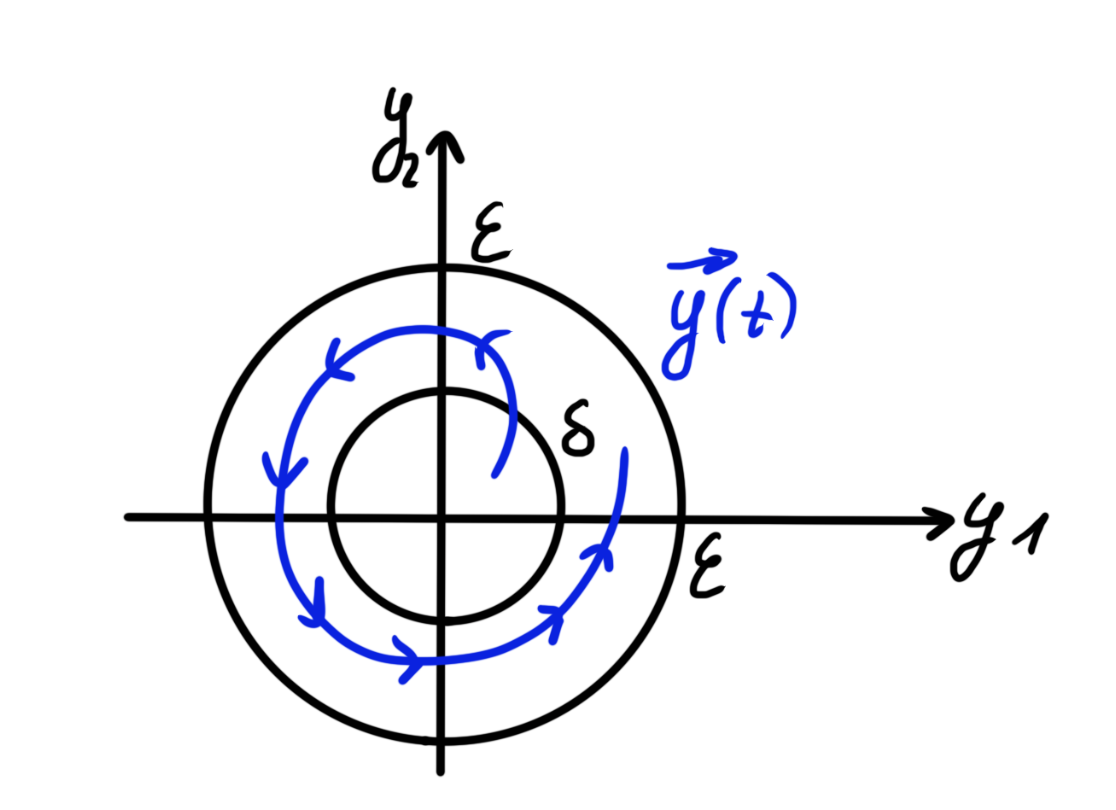
\includegraphics[width=0.3\textwidth]{/Users/vladbelousov/Desktop/Semestr_4-FP-NSU/ДфУ/Лекции_по_дням/image/48.png}
\end{center}

Предположим, что 

\begin{center}
    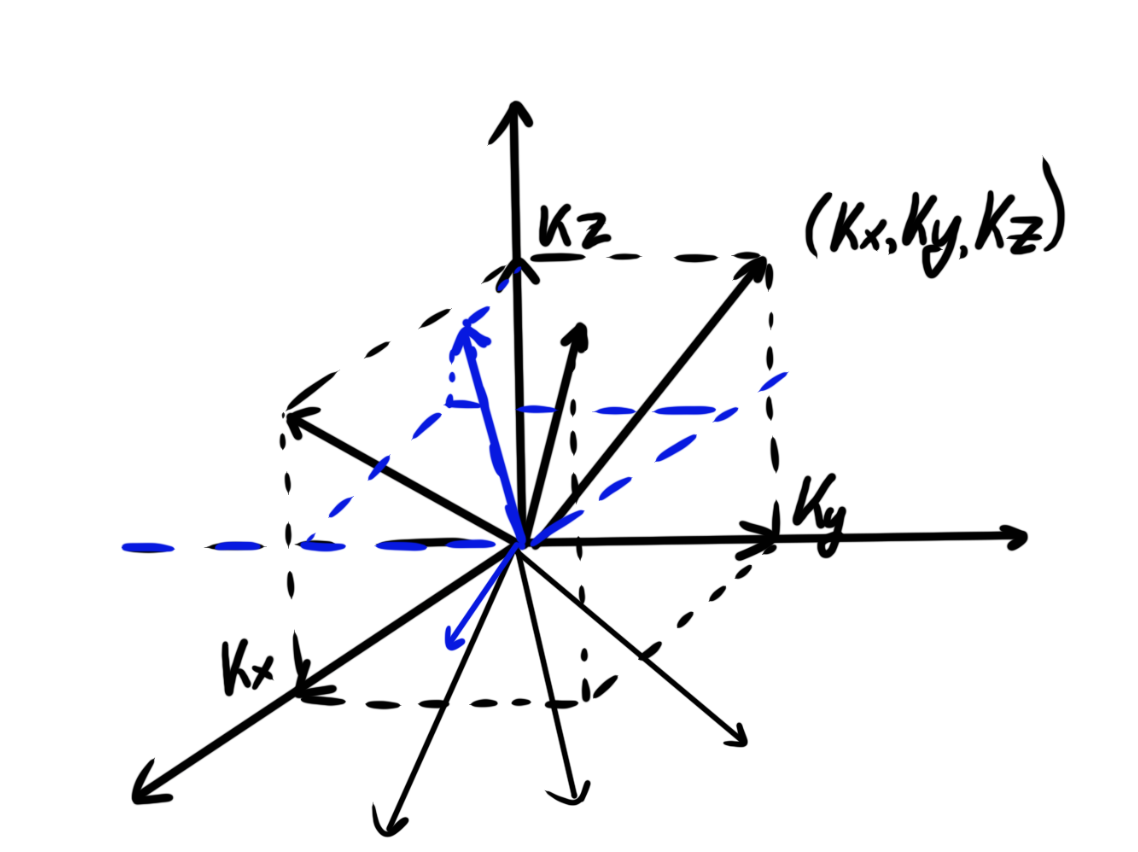
\includegraphics[width=0.55\textwidth]{/Users/vladbelousov/Desktop/Semestr_4-FP-NSU/ДфУ/Лекции_по_дням/image/49.png}
\end{center}

\[ \begin{pmatrix}
y_1(t)\\
y_2(t)
\end{pmatrix} \text{ - решение системы } \begin{cases}
y_1 ' = f_1 (y_1,y_2) \\ 
y_2' = f_2 (y_1 , y_2)
\end{cases} \] 

\begin{center}
    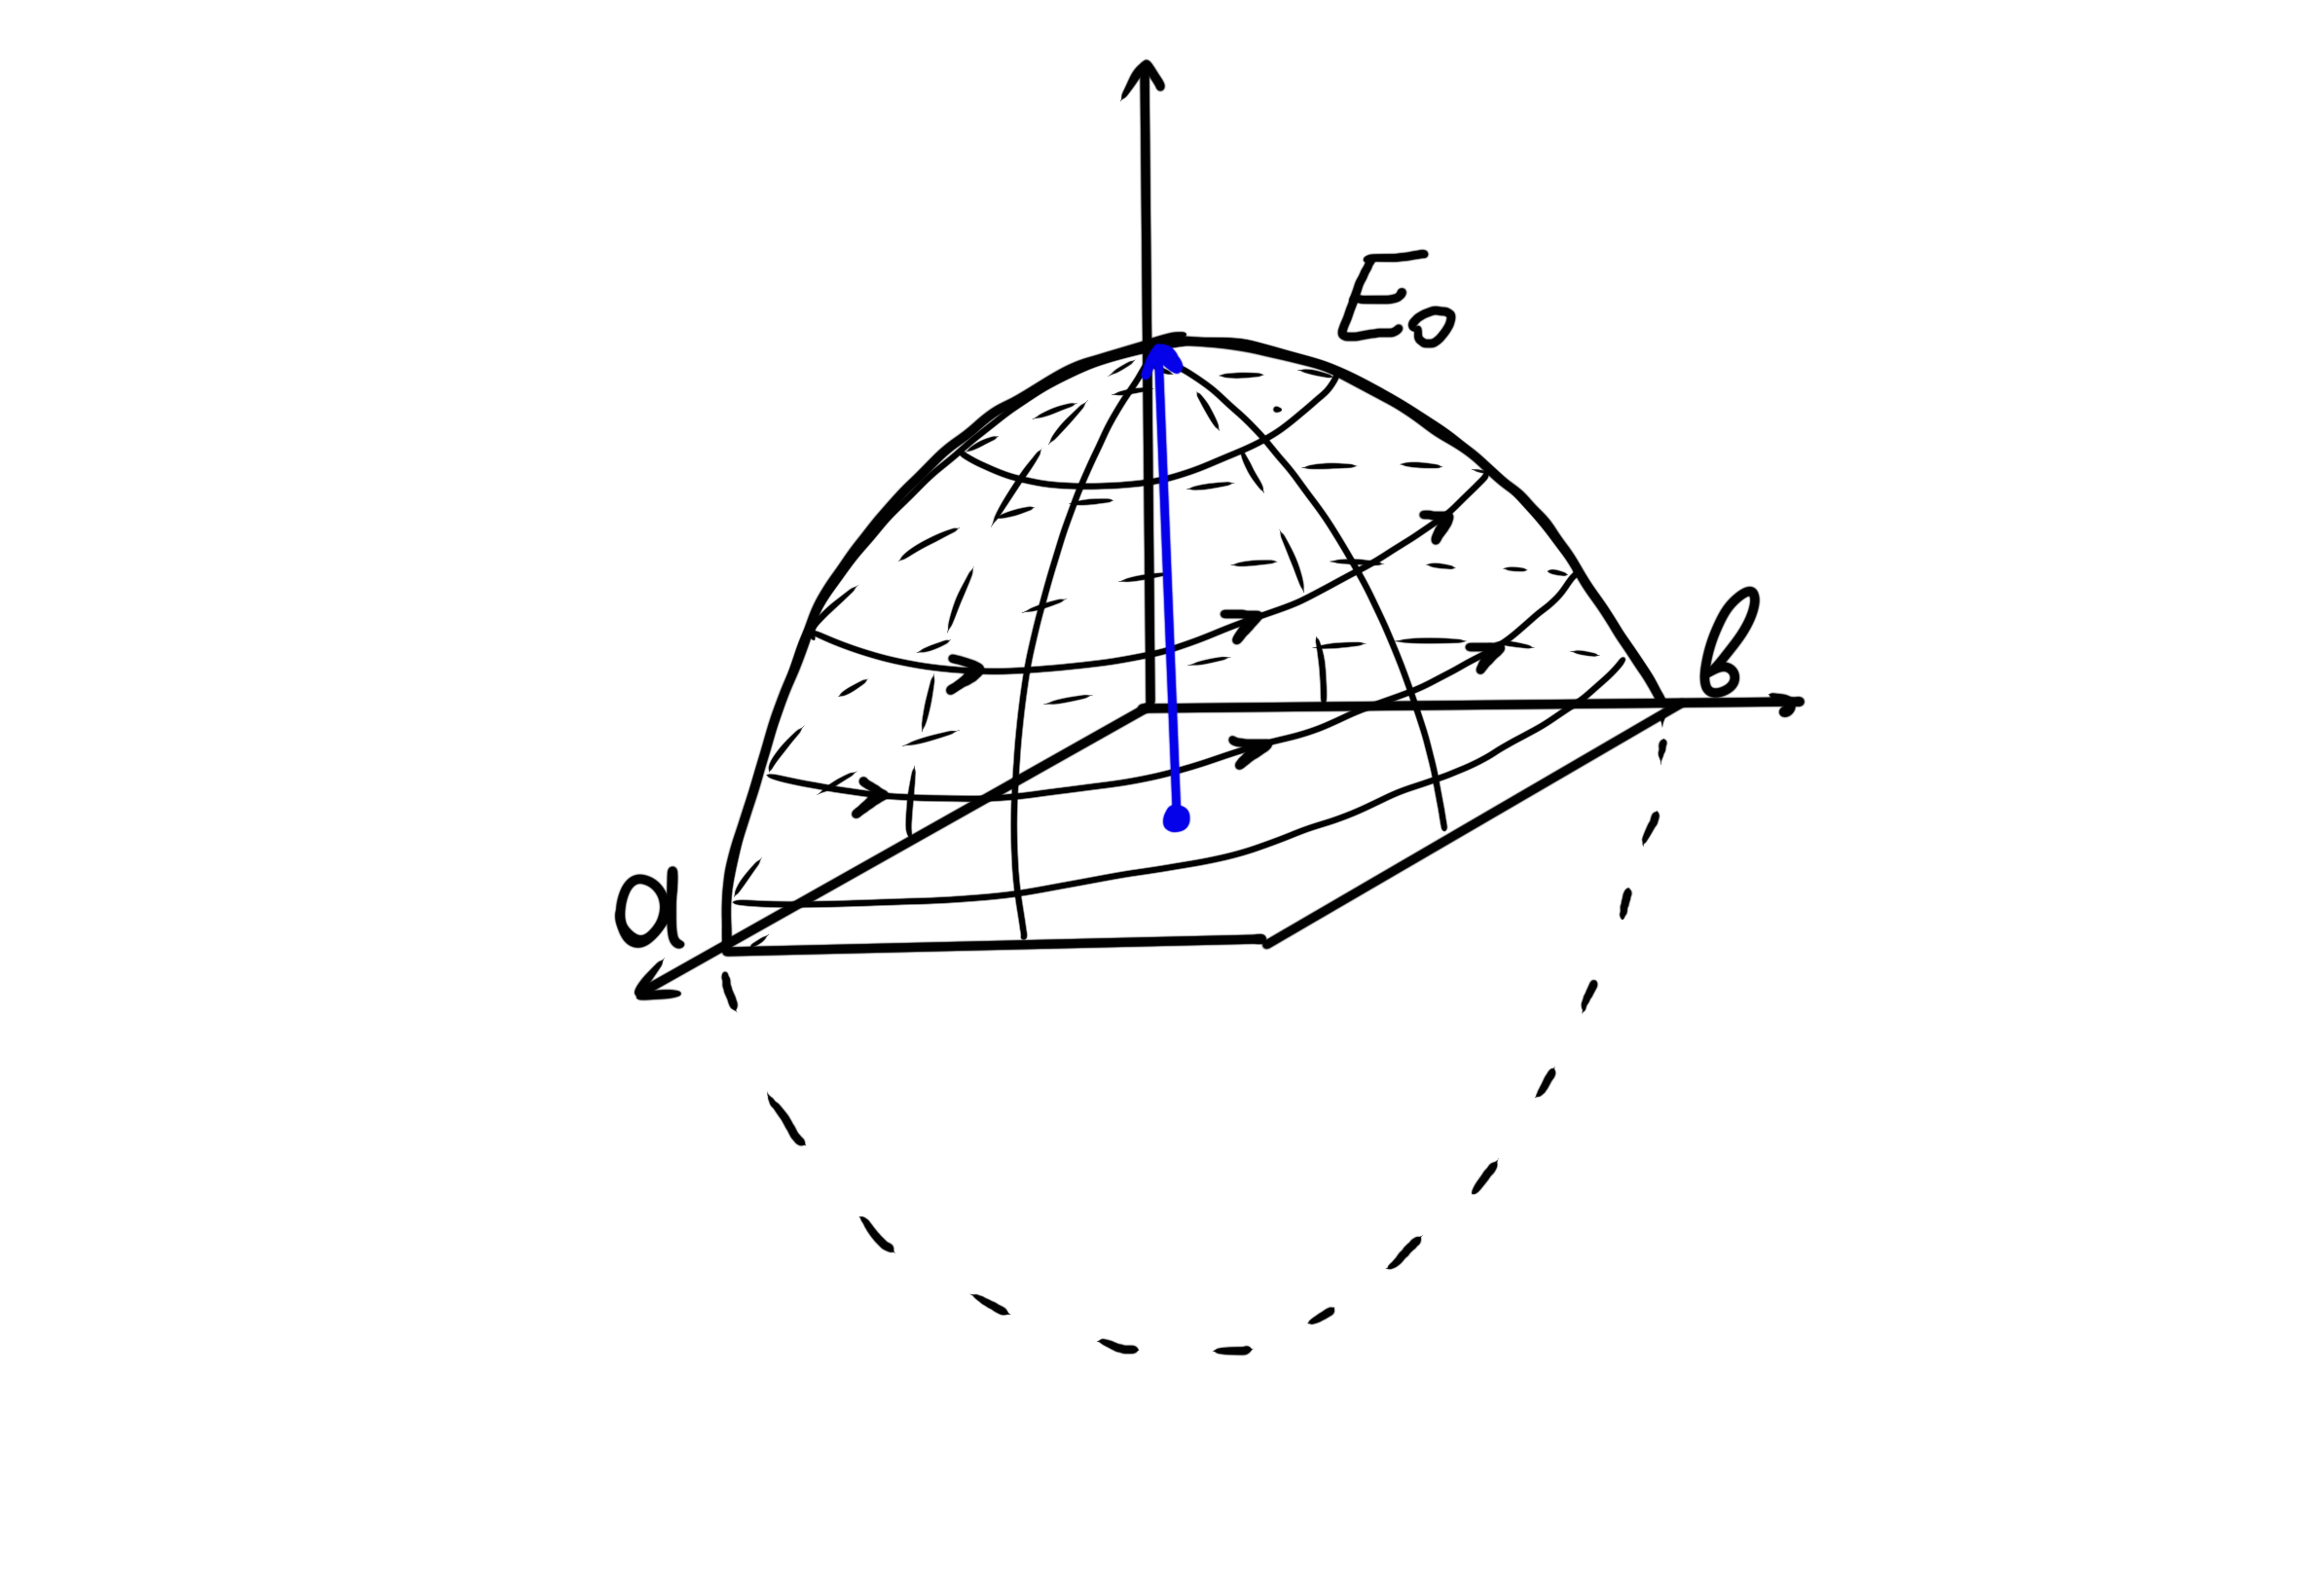
\includegraphics[width=0.3\textwidth]{/Users/vladbelousov/Desktop/Semestr_4-FP-NSU/ДфУ/Лекции_по_дням/image/50.png}
\end{center}

\[ V(y_1, y_2 ) = y_1 ^2 + y_2 ^2  = \varepsilon ^2  \] 

\[ \vec{n }  = \nabla V = \begin{pmatrix}
\displaystyle  \frac{ \partial  V }{\partial  y_1 }  \\[10pt]
\displaystyle  \frac{\partial  V }{\partial  y_2 } 
\end{pmatrix}= \begin{pmatrix}
2 y_1 \\
2 y_2 
\end{pmatrix} \] 

\( (\vec{\tau  } , \vec{n }  )< 0 \Leftrightarrow   \) угол между векторами \( \vec{\tau}  \) и \( \vec{ n}  \) от \( \displaystyle  \frac{\pi}{2 }  \)  до \( \pi \): 

\[ (\vec{\tau  } , \vec{n }  ) = \left(  \begin{pmatrix}
f_1 \\
f_2
\end{pmatrix}, \begin{pmatrix}
V _{y_1 } '  \\
V_{y_2 } ' 
\end{pmatrix} \right) = f_1 V_{y_1 } ' + f_2 V_{ y_2 } ' = f_1 2 y_1 + f_2 2 y_2 < 0   \] 

\begin{center}
    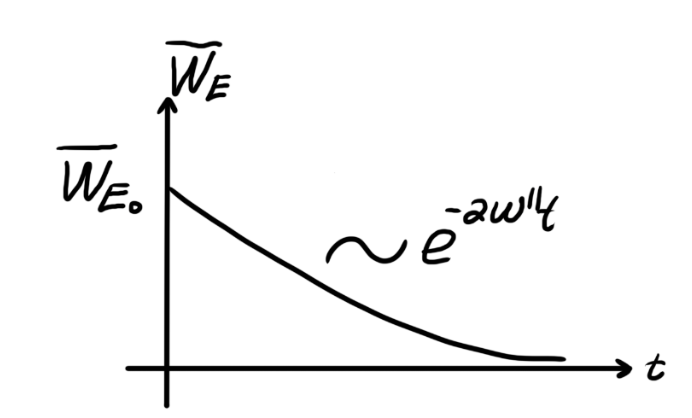
\includegraphics[width=0.4\textwidth]{/Users/vladbelousov/Desktop/Semestr_4-FP-NSU/ДфУ/Лекции_по_дням/image/52.png}
    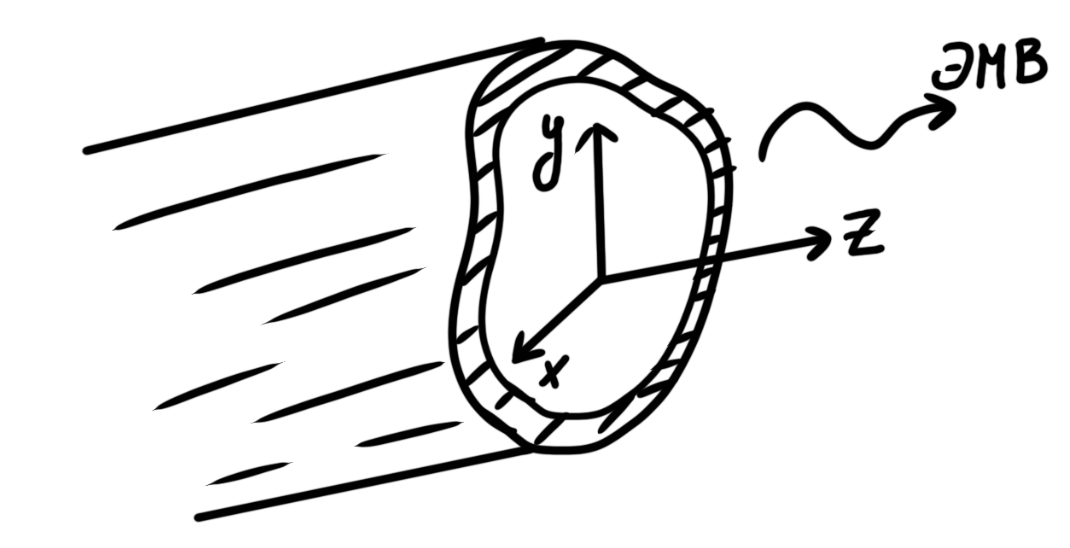
\includegraphics[width=0.4\textwidth]{/Users/vladbelousov/Desktop/Semestr_4-FP-NSU/ДфУ/Лекции_по_дням/image/51.png}
\end{center}

\begin{definition}
    Функция \( V (\vec{y }  ) \), определенная  в шаре  \( \underbrace{ \{\left\lVert \vec{y }   \right\rVert < r\}}_{\Leftrightarrow  y_1 ^2 + ... + y_n ^2 < r ^2 } \), называется функцией Ляпунова для системы (1) если: 

    1) \( V (\vec{y } ) \in  C^1 (\left\lVert \vec{y }  \right\rVert < r ) \) 

    2) \( V (\vec{y }  ) > 0 \text{ }  \forall 0 < \left\lVert  \vec{ y}  (t) \right\rVert < r , \text{ }  V(\vec{ 0 } ) =0  \) 

    3) \( (\nabla V(\vec{y } ) , \vec{f } (\vec{y } ) ) \le  0 , \text{  }  \left\lVert \vec{y }  \right\rVert < r\)
\end{definition}

\begin{theorem}[Теорема Ляпунова об устойчивости по Ляпунову]
    Если для системы (1) существует функция Ляпунова, то нулевое решение устойчиво по Ляпунову.
\end{theorem}

Пример: Исследовать на устойчивость нулевое решение. 

\[ \begin{cases}
y_1 ' = - y_1  \\ 
y_2 ' = -y_2
\end{cases} \]

1 способ: 

\[ A= \begin{pmatrix}
-1 & 0\\
0 & -1
\end{pmatrix}, \text{ }  \lambda_{1,2} = -1  \text{ }  \mathrm{Re } \lambda_j <  0 \Rightarrow \text{нулевое решение асимптотически устойчиво }    \] 

2 способ: 

\[ V (y_1 , y_2 ) = y_1 ^2 + y_2 ^2  \] 

\[ \begin{aligned}
    1)& V \in  C^1 (\mathbb{R}) \\
    2)& V > 0 , \text{ }  (y_1,y_2 ) \neq (0,0 ) , \text{ }  V (0,0 ) = 0  \\
    3)& (\nabla V , f) = \left( \begin{pmatrix}
        2y_1    \\
        2y_2
        \end{pmatrix} , \begin{pmatrix}
        -y_1\\
        -y_2
        \end{pmatrix} \right)  = -2 y_1 ^2 - 2y_2 ^2 \le  0
\end{aligned} \] 

\( \Rightarrow \)  по Теореме Ляпунова нулевое решение устойчиво по Ляпунову.

\begin{center}
    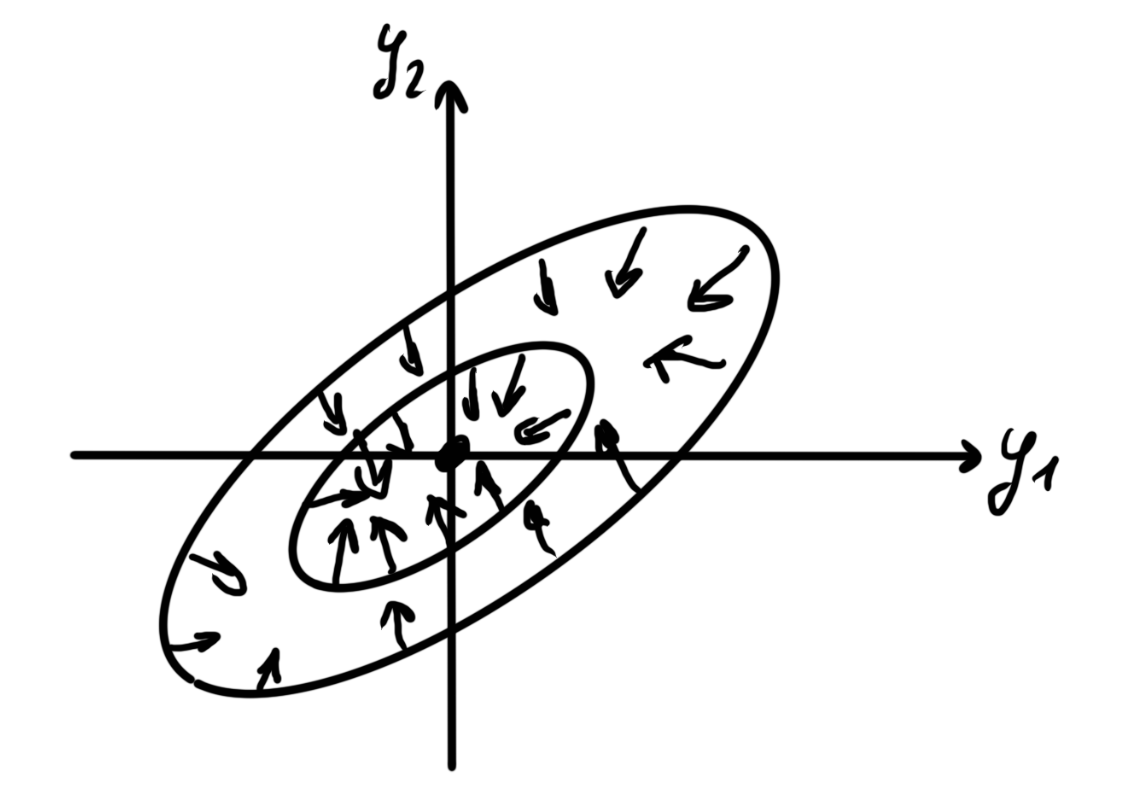
\includegraphics[width=0.4\textwidth]{/Users/vladbelousov/Desktop/Semestr_4-FP-NSU/ДфУ/Лекции_по_дням/image/53.png}
\end{center}

\begin{theorem}[Теорема Ляпунова об асимптотической устойчивости]
    Пусть существует функция \( V(\vec{y} ) \), удовлетворяет условиям 1), 2), \( 3^*)  \text{ }  (\nabla V(\vec{y} ), \vec{f } (\vec{y } ))< 0\) при \( 0 < \left\lVert \vec{y }  \right\rVert < r \). Тогда нулевое решения \( \vec{y } ^* (t) =0  \) асимптотически устойчиво.
\end{theorem}

\begin{theorem}[Теорема Ляпунова об асимптотической неустойчивости]
    Пусть существует функция \( V(\vec{y} ) \) удовлетворяющее условиям 1), 2), \( 3^{**}) (\nabla V(\vec{y } ) , \vec{f } ( \vec{y } )) > 0  \) при \( 0 < \left\lVert  \vec{y }  \right\rVert < r \). Тогда нулевое  решение неустойчиво.
\end{theorem}
%%-------------------------------%%

% Закрытие документа, если файл компилируется отдельно
\ifdefined\mainfile
    % Если это основной файл, не нужно заканчивать документ
\else
    \end{document}
\fi